\documentclass[12pt]{amsart}
\usepackage{geometry}                % See geometry.pdf to learn the layout options. There are lots.
\geometry{letterpaper}                   % ... or a4paper or a5paper or ... 
%\geometry{landscape}                % Activate for for rotated page geometry
%\usepackage[parfill]{parskip}    % Activate to begin paragraphs with an empty line rather than an indent
\usepackage{graphicx}
\usepackage{amssymb}
\usepackage[all]{xy}
\usepackage{epstopdf}
\usepackage{geometry}
\geometry{legalpaper, portrait, margin=1in}

\DeclareGraphicsRule{.tif}{png}{.png}{`convert #1 `dirname #1`/`basename #1 .tif`.png}


% these packages make it easy to include figures in the text. 
\usepackage{float}
\restylefloat{figure}

\newcommand{\lt}{\left}
\newcommand{\rt}{\right}
\newcommand{\la}{\lt\langle}
\newcommand{\ra}{\rt\rangle}
\newcommand{\ip}[1]{\la #1 \ra}
\newcommand{\T}{^{\mathsf{T}}}
\newcommand{\R}{\mathbb{R}}
\newcommand{\E}{\mathbb{E}}
\newcommand{\cX}{\mathcal{X}}
\newcommand{\cC}{\mathcal{C}}
\newcommand{\cF}{\mathcal{F}}

\DeclareMathOperator*{\argmin}{argmin}

% Path for the graphics
\graphicspath{ {../R/Graphs/} }

\begin{document}
{\bf \Large AMATH 521 Final Project}\\
\begin{center}
{\bf \Large Topic: Sector Outperformance Analysis}\\
\end{center}
\vskip 16pt \noindent
{\textbf{Contributors}: }
\vskip 8pt \noindent
1.) Luke Lee\\
2.) Wipada Wannasiwaporn

\vskip 8pt \noindent
{\textbf{Summary}: }
\vskip 8pt \noindent
The goal of this project was to build a model that predicts the sectors that tend to outperform the market return using logistic regression with different penalties and try out different models for comparison. In order to confine our scope of the project, we decided to focus on the two largest sector in S\&P500, Technology and Financial. 

%==============================================
\vskip 8pt \noindent
{\textbf{Data}: }
\vskip 8pt \noindent
Our independent variables are basically the monthly macro economics data retrieved from FRED(https://fred.stlouisfed.org/). Some examples of these data are unemployment 
rate, FED funds rate, CPI, SP500 monthly return etc. We also added some sector related data such as Telecommunication export, (TODO: Financial Related)... to possibly add prediction power for a specific sector as well. We convert these raw data into a return space using monthly simple return for an Index-like data and use percentage conversion for a probability data and rate data. Here are some samples of our data.\\

% Table generated by Excel2LaTeX from sheet 'tech_raw_data'
\begin{table}[htbp]
	\centering
	\caption{Data Example}
	\begin{tabular}{rrrrrrr}
		\multicolumn{1}{l}{Date} & \multicolumn{1}{l}{IYW return} & \multicolumn{1}{l}{GDP} & \multicolumn{1}{l}{CSUSHPINSA} & \multicolumn{1}{l}{DGS10} & \multicolumn{1}{l}{TEDRATE} & \multicolumn{1}{l}{FEDFUNDS} \\
		10/31/2000 & -0.080775444 & 0.011088 & 0.005507 & 0.0577 & 0.0057 & 0.0651 \\
		11/30/2000 & -0.234329233 & 0.011088 & 0.005198 & 0.0548 & 0.0068 & 0.0651 \\
		12/31/2000 & -0.087222647 & 0.011088 & 0.004617 & 0.0512 & 0.0067 & 0.064 \\
		01/31/2001 & 0.172170997 & 0.003422 & 0.003953 & 0.0519 & 0.0056 & 0.0598 \\
	\end{tabular}%
	\label{tab:addlabel}%
\end{table}%
\vskip 8pt \noindent
For the dependent variable, we use a separate model for each sector.\\

\textbf{i)} For Technology Sector, we use BlackRock's ETF(IYW) that tracks the Technology sector performance using Dow Jones as a benchmark. Overall, the returns of Technology sector moves strongly correlated with the return of S\&P500 as seen in the high correlation value.
\begin{center}
	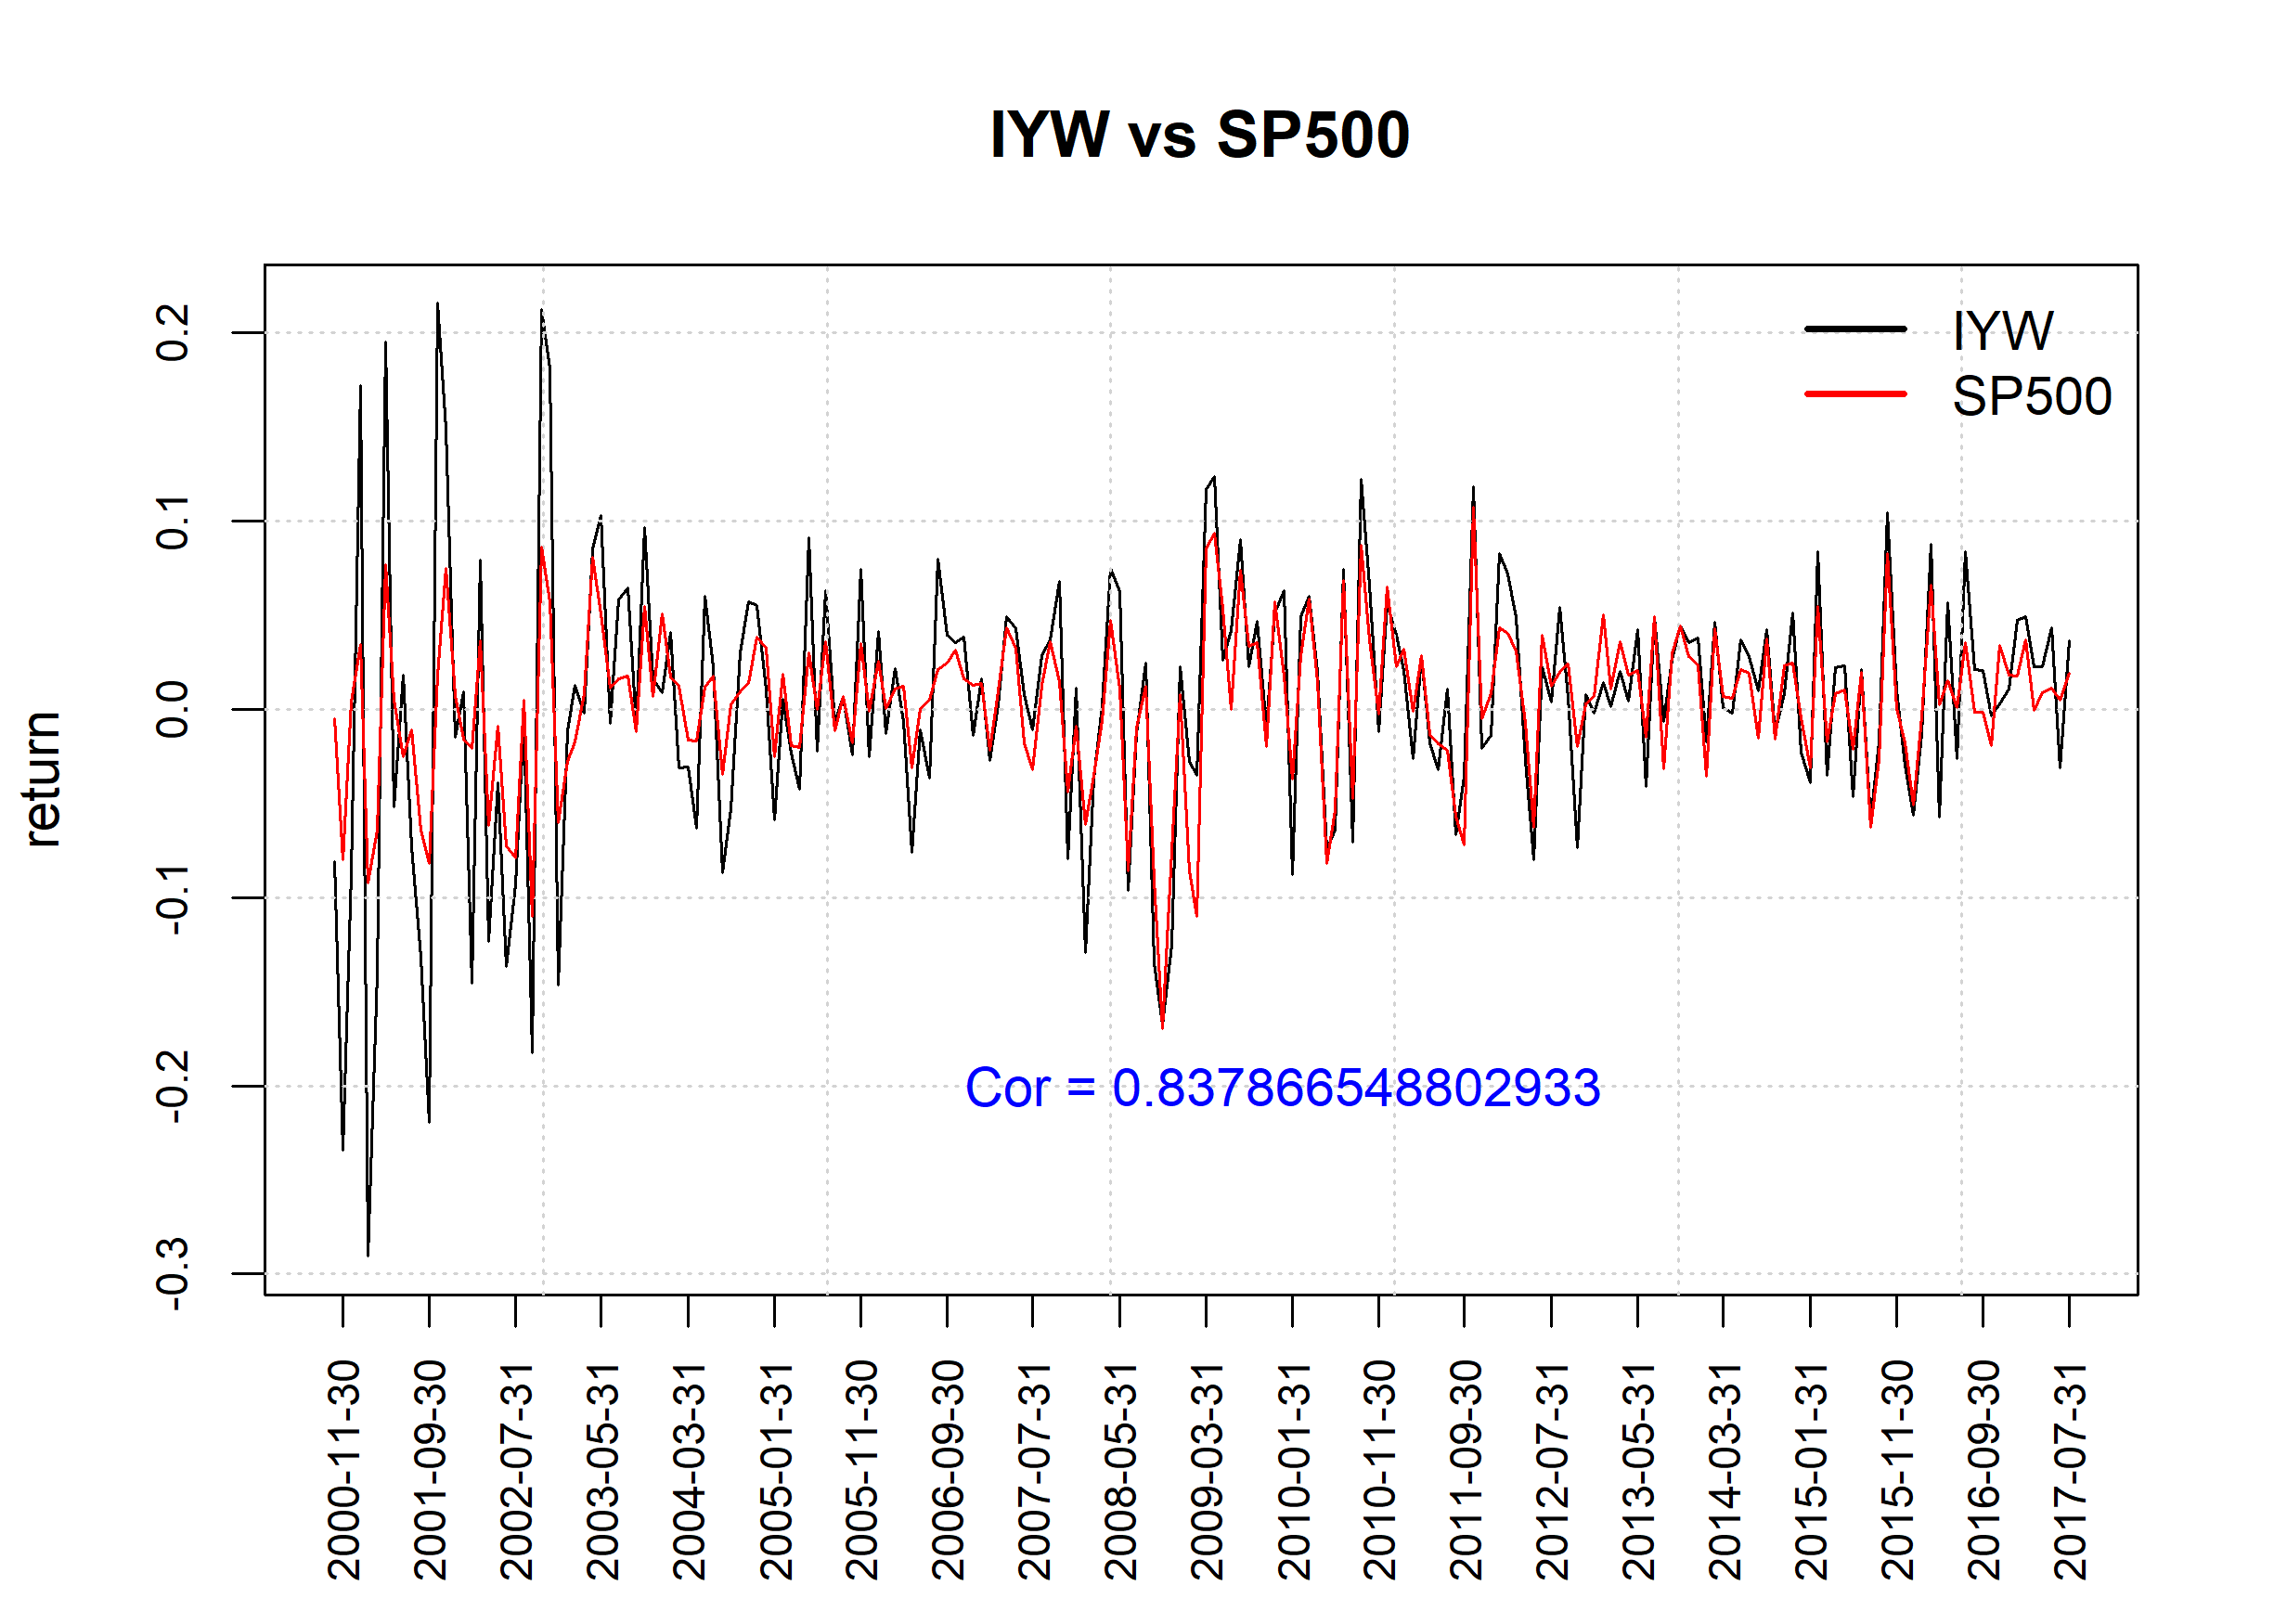
\includegraphics[scale=0.7]{IYW_vs_SP500}
\end{center}

\textbf{ii)} For Financial Sector,
\vskip 8pt \noindent

%==============================================

\newpage

\vskip 8pt \noindent
{\textbf{Methods \& Algorithms}: }
\vskip 8pt \noindent

\textbf{i)} Linear Regression\\
We first want to make sure that our data can explain the data well, so doing linear regression is one way of doing sanity check on our data. It turns out that the explained variance($R^{2}$) is quite high for this data set, so we know our independent variables can somehow explain our dependent variable.

\begin{center}
	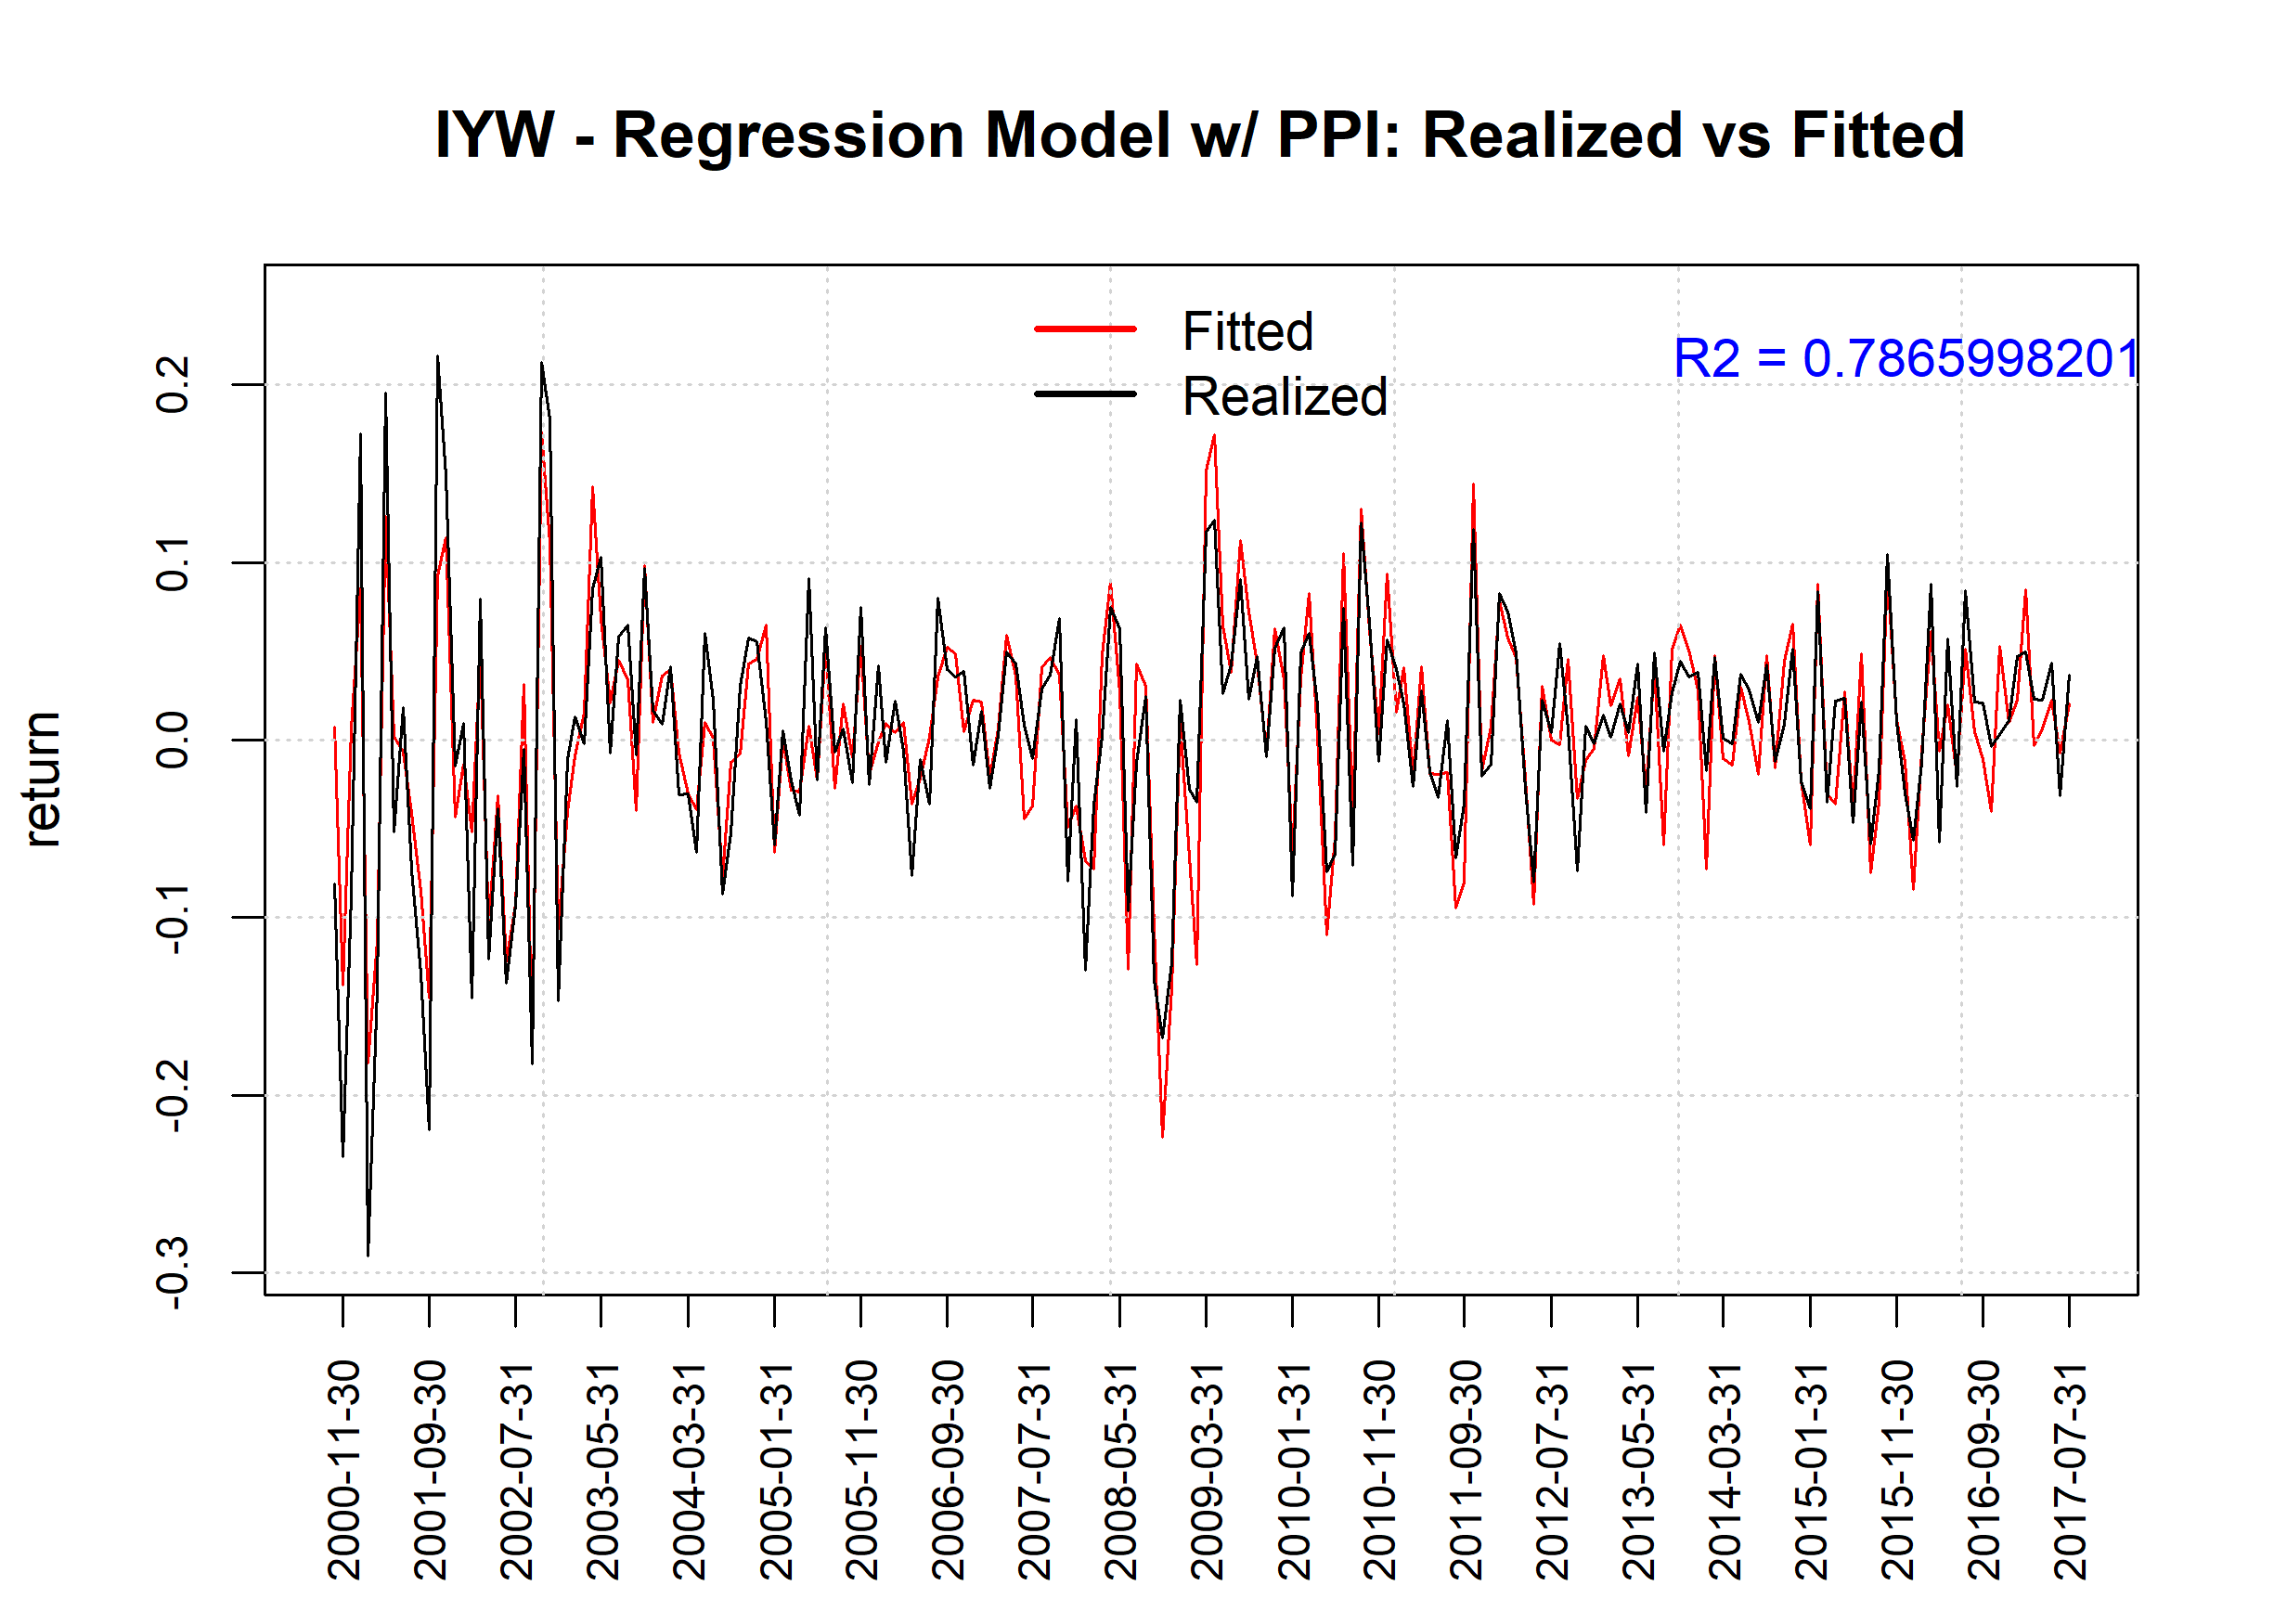
\includegraphics[scale=0.7]{IYW_linear_reg_withPPI}
\end{center}

\textbf{ii)} Logistic Regression\\

\textbf{iii)} Logistic Regression with Elastic Net\\

\textbf{iv)} Support Vector Machine\\


\end{document}  
